% 2002 年春季京蒙皖理卷第 19 题：三棱锥空间图形
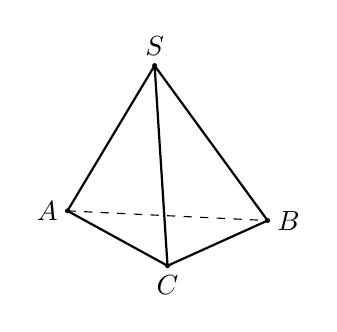
\begin{tikzpicture}[>=stealth, scale=0.82]
  \coordinate (A) at (0,0);
  \coordinate (C) at (1.55,-0.85);
  \coordinate (B) at (3.1,-0.15);
  \coordinate (S) at (1.35,2.25);

  \draw[thick] (A)--(C)--(B);
  \draw[dashed] (A)--(B);
  \draw[thick] (S)--(A) (S)--(B) (S)--(C);

  \fill (A) circle (1.1pt) node[left] {$A$};
  \fill (B) circle (1.1pt) node[right] {$B$};
  \fill (C) circle (1.1pt) node[below] {$C$};
  \fill (S) circle (1.1pt) node[above] {$S$};
\end{tikzpicture}
